%# -*- coding:utf-8 -*-
\documentclass[10pt,aspectratio=169,mathserif]{beamer}		
%设置为 Beamer 文档类型,设置字体为 10pt,长宽比为16:9,数学字体为 serif 风格

%%%%-----导入宏包-----%%%%
\usepackage{hit}			%导入 CCNU 模板宏包
\usepackage{ctex}			%导入 ctex 宏包,添加中文支持
\usepackage{amsmath,amsfonts,amssymb,bm}   %导入数学公式所需宏包
\usepackage{color}			 %字体颜色支持
\usepackage{graphicx,hyperref,url}
\usepackage{metalogo}	% 非必须
\usepackage{color}
%% 上文引用的包可按实际情况自行增删
%%%%%%%%%%%%%%%%%%	


\beamertemplateballitem		%设置 Beamer 主题

%%%%------------------------%%%%%
\catcode`\。=\active         %或者=13
\newcommand{。}{.}				
%将正文中的“。”号转换为“.”。中文标点国家规范建议科技文献中的句号用圆点替代
%%%%%%%%%%%%%%%%%%%%%

%%%%----首页信息设置----%%%%
\title[开关电源设计开发实践与创新思维课程报告]{开关电源设计开发实践与创新思维课程报告}
\subtitle{——交错串联电容分接Buck降压电路 \ ISC-TaB}			
%%%%----标题设置


\author[W.J.C]{
  王浩瑞 \ 蒋佳诚 \ 曹广旭 \\\medskip
  {\small \url{1180610825@stu.hit.edu.cn}} \\
  {\small \url{url}}}
%%%%----个人信息设置
  
\institute[IOPP]{
  电气工程及自动化学院 \\ 
  }
%%%%----机构信息

\date[Oct. 20 2020]{
  2020年10月20日}
%%%%----日期信息
  
\begin{document}

\begin{frame}
\titlepage
\end{frame}				%生成标题页

\section{提纲}
\begin{frame}
\frametitle{提纲}
\tableofcontents
\end{frame}				%生成提纲页

\section{背景}
\begin{frame}
  \frametitle{背景}

  \begin{itemize}
    \item 通讯、工业系统用电需要做到高低压隔离
	    \begin{itemize}
	    	\item DC/DC变换器
	    	\item 如何实现高降压比?
	    \end{itemize} 
	\item Buck电路及其拓扑
	 \begin{itemize}
		\item SC-Buck
		\item Buck-Boost
		\item \textcolor{red}{ISC-Buck}
	\end{itemize} 
  \end{itemize}
\end{frame}

\begin{frame}
	\frametitle{参考电路图}
	\begin{columns}[T] % align columns
		\begin{column}<0->{.70\textwidth}
			\begin{figure}[thpb]
				\centering
				\resizebox{1\linewidth}{!}{
					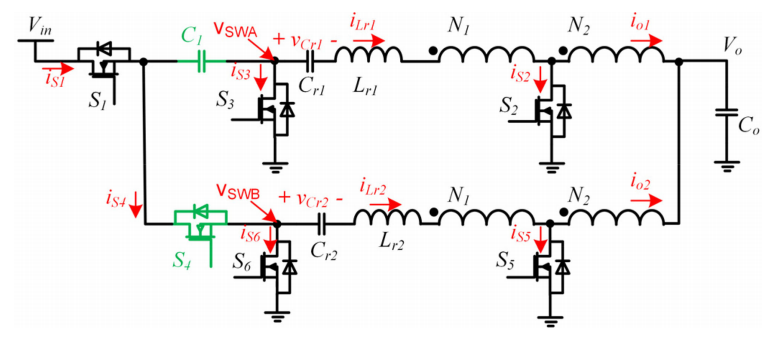
\includegraphics{figure/circuit diagram1.png}
				}
				%\includegraphics[scale=1.0]{figurefile}
				\caption{参考电路图}
				\label{fig:campus}
			\end{figure}
    \end{column}%
    \begin{column}<0->{.70\textwidth}
			\begin{itemize}
        \item 123456
      \end{itemize}
    \end{column}%
	\end{columns}
\end{frame}

\begin{frame}
  \frametitle{仿真电路图}
  \begin{columns}[T] % align columns
		\begin{column}<0->{.70\textwidth}
			\begin{figure}[thpb]
				\centering
				\resizebox{1\linewidth}{!}{
					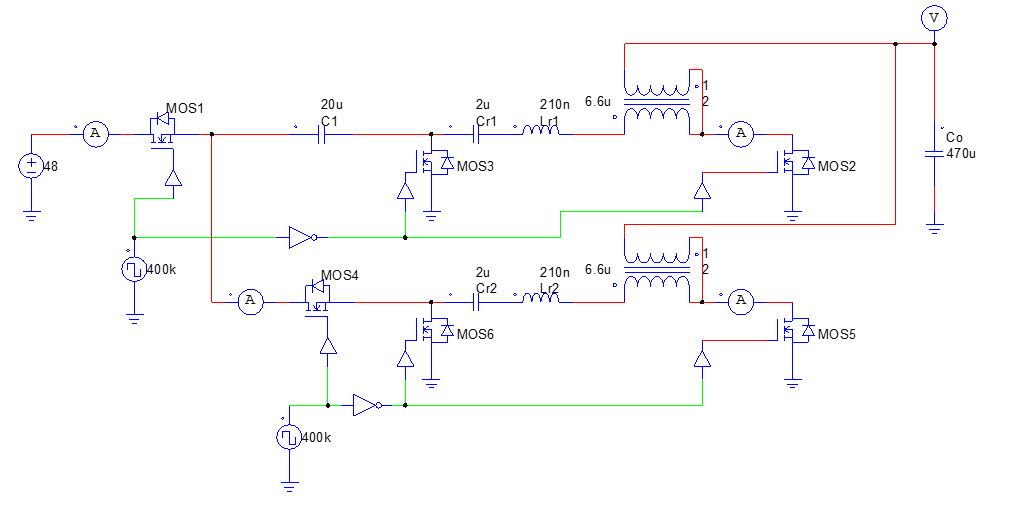
\includegraphics{figure/PSIM-circuit diagram1.png}
				}
				%\includegraphics[scale=1.0]{figurefile}
				\caption{参考电路图}
				\label{fig:campus}
			\end{figure}
    \end{column}%
    \begin{column}<0->{.70\textwidth}
			\begin{itemize}
        \item 123456
      \end{itemize}
    \end{column}%
	\end{columns}
\end{frame}

\section{电路原理}
\begin{frame}
  \frametitle{电路原理}

  \begin{itemize}
    \item Easy to use
    \item Good results
  \end{itemize}
\end{frame}

\section{仿真结果}
\begin{frame}
  \frametitle{仿真结果}

  \begin{itemize}
    \item Easy to use
    \item Good results
  \end{itemize}
\end{frame}

\section{结论/思考}
\begin{frame}
  \frametitle{结论/思考}

  \begin{itemize}
    \item Easy to use
    \item Good results
  \end{itemize}
\end{frame}

\section{参考文献}
\begin{frame}{参考文献}
\begin{thebibliography}{99} 
\bibitem{zhao1} Yi~Zhao, {\sl An introduction to X}, Sep.~15, 2015
\bibitem{qian2} Er~Qian, San~Sun, 
Phys.\ Lett.\ A {\bf xx}, 2xx (20xx)   
\bibitem{li4} Si~Li, Phys.\ Rev.\ C {\bf xx}, 5xx (20xx) 

\end{thebibliography}
\end{frame}




\end{document}